% -*-mode: Latex-*-
% !TEX root = thesis.tex
% paper: ...
% authors: simon maurer
%
% file: streamix.tex
% contents: Streamix our coordination language
% Sccs-Id: %W% %G%
\chapter{Streamix - An Instantiation of PNSCs as a Coordination Language}
\label{chap_smx}
In this chapter I introduce the coordination language \gls*{smx}.
\Gls*{smx} is based on the \gls{pnsc} model which I introduced in \Chap{\ref{chap_ecm}} and extended in \Chap{\ref{chap_tcm}}.
Therefore, \gls*{smx} represents one possible instance of the \gls{pnsc} model and serves as proof of concept.

The inspiration for \gls*{smx} stems from the coordination language \gls*{snet}~\cite{grelck2010}.
One of the achievements of \gls*{snet} is the capability of modelling networks in a structured manner by employing binary operators.
\Gls*{smx} adopts the concept of structured programming and uses similar operators to model networks.
The concept of the underlying model of \gls*{smx}, however, differs largely from \gls*{snet} due to the differences of their respective targeted application fields.
While \gls*{smx} is suitable for \glspl{cps}, where complex, reactive interaction patterns pose a challenge for structured system composition, \gls*{snet} is mostly intended for best-effort applications with transformational data-processing aspects (\eg systems where computational chunks can easily be pipelined).

Structured programming has become a very successful programming paradigm as it provides locality of a program's control flow.
Similar concepts of locality are desired for the specification and development of concurrent and parallel systems.
In the domain of \glspl{cps} or embedded computing it is challenging to identify such structured compositions since control flow tends to be driven by concurrently acting reactive components with often circular dataflow relations.

A structured network provides a sense of locality and allows to observe and understand a part of the network without having to consult other, potentially distant, parts of the network.
This is achieved by keeping port-to-port connections local.
In contrast to this, a non-structured network would rather be created with global port-to-port connection tables which are hard to read and understand.
For a modular development it is important to understand the behaviour of an isolated sub-entity, independent of where it is going to be integrated, which is why a structured approach is key.

\Gls*{smx} aims to enforce structure, support reactive data processing, and allow persistent state and synchronisation points within behavioural components.
\Gls*{smx} allows to model streaming networks where the topology of the network imposes dependencies between components and where message streams are coordinated within the network.
\Gls*{smx} is a representative of the exogenous coordination model~\cite{arbab2006} in order to assure clear separation of concerns.

The chapter is structured as follows:
\Sect{\ref{sect_smx_model}} gives an overview of the coordination model of the language which consists of three layers, namely the \glspl*{ccomp}, the \gls*{rnw}, and the \gls*{efrl}.
\Sect{\ref{sect_smx_box}} describes the box abstraction, an abstraction used to represent \glspl*{ccomp}.
\Sect{\ref{sect_smx_nets}} describes how such boxes are instantiated as nets and how their interface is defined.
\Sect{\ref{sect_smx_network}} describes how to compose multiple nets with different network operators.
Finally, in \Sect{\ref{sect_smx_conclusion}} I discuss limitations of the coordination language and in \Sect{\ref{sect_smx_summary}} I summarise the chapter.

% In Section \ref{sect.nets} we introduce the underlying coordination model and in Section \ref{sect.op} we describe network operators.
% Section \ref{sect.example} presents an example of a CPS where we apply the presented coordination concepts.
% Section \ref{sect.related_work} discusses related work and Section \ref{sect.conclusion} concludes the dissertation.

% In this dissertation we discuss foundations for a structured coordination language for cyber-physical systems.
% We study car platooning as a use case, exhibiting typical challenges of cyber-physical systems.
% Based on that use case we show a possible structured composition pattern and outline coordination network construction mechanisms.

% %------------------------------------------------------------------------------
% \subsection{Structured Programming}
% \label{sect_smx_cps_struct}
% A straight forward approach to implement a streaming network, while respecting the concerns raised above, would be a point-to-point connection scheme of computational components by streams.
% However, such a scheme can become very complex and very hard to maintain due to the lack of structure.
% By using network operators, a structuring of the network and hence, of the coordination program is achieved.

% Structured in general means some sense of locality (c.f., structured programming, etc.).
% We may argue that locality can be helpful to get better Composability and Compositionality \footnote{\url{http://homepages.herts.ac.uk/~rk10aah/papers/rr-2009-014_isorc-stfssd09_composable_timing.pdf}}.

% The following Section describes the network components and operators in detail.

%==============================================================================
\section{Coordination Model}
\label{sect_smx_model}
% To describe the concept of coordination I start at the beginning and consider the necessary mechanisms to run an application on a parallel hardware architecture.
An application can benefit from a parallel hardware architecture if it is decomposable into multiple chunks, called \emph{\glspl*{ccomp}} throughout the chapter, where some or all of those can be run, possibly at the same time, on different parts of the parallel architecture.
The \glspl*{ccomp} may be required to interact with each other which must be handled by some sort of communication structure, called \emph{\gls*{rnw}} throughout the chapter.
A \gls*{rnw} can be a simple connection between two \glspl*{ccomp} or it can include complex synchronisation and routing operations to coordinate multiple \glspl*{ccomp}.
If the decomposition is performed to such a granularity that the only concern of one \gls*{ccomp} is to execute a specific functionality and all communication and synchronisation of data happens through \glspl*{rnw} placed outside the \gls*{ccomp}, perfect separation of concerns with respect to behaviour and coordination is achieved.
\Gls*{smx} does not require such a decomposition as it targets \glspl{cps} where \glspl*{ccomp} are often of reactive nature which are hard to decompose~\cite{harel1985}.
The separation is further underlined by using a conventional programming language to describe the behaviour of the content of a \gls*{ccomp} and a coordination language to describe the \glspl*{rnw}.

To summarize, the general coordination model described above consists of \emph{\glspl*{ccomp}}, \emph{\glspl*{rnw}}, and an \emph{\gls*{efrl}}.
% This is schematically depicted in \Fig{\ref{fig_smx_model}}.
In the following each layer is described in more detail.

%------------------------------------------------------------------------------
\subsection{Computational Components}
\label{sect_smx_model_ccomp}
The \glspl*{ccomp} are oblivious of any other \gls*{ccomp} and also to the fact that they are coordinated by \glspl*{rnw}.
This corresponds, according to the classification of Arbab~\cite{arbab1998}, to an exogenous coordination model.
\Glspl*{ccomp} follow a triggering semantics that is imposed by the coordination model but they are not altered by the coordination language in any way.
A \gls*{ccomp} is considered to be a black box by the coordination language and can have persistent state or be stateless (pure).
% The behaviour of a \gls*{ccomp} is described by a separate programming language.

%------------------------------------------------------------------------------
\subsection{Routing Network}
\label{sect_smx_model_rnw}
The concerns of the coordination language are the synchronisation and routing of information that is passed between \glspl*{ccomp} through \glspl*{rnw}.
In this chapter, any information or data that is transmitted over a \gls*{rnw} will be referred to as \emph{\gls*{msg}}, independent of the complexity or the type of the information.
\Glspl*{rnw} can be composed out of multiple primitives to form a complex coordination construct.
Such primitives are referred to as \emph{\glspl*{ocomp}} throughout this chapter.
\Glspl*{ocomp} can be either implicitly generated or explicitly described by the coordination language.
In the latter case, the coordination language defines primitives to perform explicit coordination actions within the coordination model.
Common examples are \glspl*{ocomp} that perform synchronization, copy, or merge operations.
The most basic \gls*{ocomp} is a channel, where \glspl*{msg} are transmitted from one end to the other with an implicit synchronisation between the two ends.
Channels are buffered and follow the \emph{First In, First Out (FIFO)} principle.
The \glspl*{rnw} serve as coordination instances between \glspl*{ccomp} that glue the \glspl*{ccomp} together and are hence the glue-code between the \glspl*{ccomp}.

%------------------------------------------------------------------------------
\subsection{Extra-functional Requirements Layer}
\label{sect_smx_model_efrl}
Another aspect of coordination is the question \emph{when} the \glspl*{ccomp} are executed.
This depends on the data dependencies between the \glspl*{ccomp} but also on the time-criticality of the system.
Data dependencies are given out of construction by the network topology.
For \glspl*{ccomp} without particular timing constraints, the scheduler of the runtime system of the coordination model decides when \glspl*{ccomp} are executed.
This is also true in the case of time-critical systems, however, when deadlines must be respected the scheduler is not only influenced by the data dependencies but also by imposed timing requirements on the \glspl*{ccomp}.
Such timing requirements are provided by the third layer of the language architecture, the \emph{\gls*{efrl}}.
In general, the \emph{\gls*{efrl}} allows to annotate \glspl*{ccomp} or \glspl*{rnw} in order to ensure requirements that are linked to the extra-functional behaviour of the coordination of the application.

%==============================================================================
\section{Box Abstraction}
\label{sect_smx_box}
In order do describe how a \gls*{ccomp} interacts with \glspl*{ocomp}, it is associated to a construct I call \emph{box} throughout this chapter.
A box has input and output ports, corresponding to the input and output parameters of a \gls*{ccomp}.
A box is of type \gls{mimo}.
I use the term \emph{mode} of a port to talk about its direction, \ie whether it is an input or an output port.
Further, a \gls{sia} is associated with a box.
While the \gls*{ccomp} describes the behaviour of the box, a \gls{sia} describes the interaction of the box with its environment.

Boxes need to be instantiated.
An instance of a box is called a \emph{net} in \gls*{smx}.
Similar to a class in an object-oriented programming language serving to create objects, a box in \gls*{smx} serves as a code template to create nets.
A net corresponds to a process of a \gls{pnsc} as defined by \Def{\ref{def_proc}}.
Nets are hierarchical and can include other nets and networks of nets.
This is further discussed in \Sect{\ref{sect_smx_nets}}.

%------------------------------------------------------------------------------
\subsection{User-defined Boxes}
\label{sect_smx_box_user}
Boxes are either user-defined or fulfil a predefined function.
User-defined boxes serve as an abstraction for \glspl*{ccomp} that describe a custom functionality of an application.
Such \glspl*{ccomp} are usually provided by a domain expert and implemented in a programming language suitable for the specific problem.

A user-defined box is declared and assigned to a symbol which can later be used to spawn a net instance of the declaration.
A box declaration links the source code of a \gls*{ccomp} to the box and assigns the input and output parameters of the \gls*{ccomp} with the input and output ports of the box.
For example, the following box declaration links the input parameter \texttt{x} and the output parameter \texttt{y} of the \gls*{ccomp} \texttt{fa} to the input port \texttt{x} and output port \texttt{y} of the box \texttt{A}.
\begin{lstlisting}[numbers=none]
A = box fa( in x, out y )
\end{lstlisting}

The names of the \gls*{ccomp} parameters must not necessarily be the same as the names of the corresponding box ports.
If so, this must be specified in the box declaration.
In the following example, the parameters \texttt{x} and \texttt{y} of \gls*{ccomp} \texttt{fa} are linked to the ports \texttt{x\_box} and \texttt{y\_box} of box \texttt{B}.
\begin{lstlisting}[numbers=none]
B = box fa( in x_box( x ), out y_box( y ) )
\end{lstlisting}
This allows to reuse the same \gls*{ccomp} in a different environment by declaring a new box and assigning it to a different symbol.

%------------------------------------------------------------------------------
\subsection{Implicit Boxes}
\label{sect_smx_box_implicit}
In \Chap{\ref{chap_ecm}} I introduced an interface model, called \gls{sia}, that allows to describe the interaction of processes with their environment.
In \Chap{\ref{chap_block}} I then introduced an analysis based on \glspl{sia} that allows to check for freedom of permanent blocking within the process network.
\Glspl{sia} are part of the \gls{pnsc} model where two basic primitives are used to model an application: processes and synchronous channels.
The model offers a separation of computational and coordination concerns by describing an application as a network of processes where processes represent \glspl*{ccomp} and channels, connecting processes, represent \glspl*{ocomp}.
In \Chap{\ref{chap_tcm}} I extended the model with \glspl{cci} that allow coordination of processes with respect to communication coupling or rate-control.
% However, the separation is only marginal because the coordination capabilities of channels are limited to the implicit synchronization between to linked processes.
\Gls*{smx} implements \glspl{cci} as \glspl*{ocomp} and provides more implicitly generated \glspl*{ocomp}.
In this section I will describe these \glspl*{ocomp} that serve to route and synchronize \glspl*{msg} in the network.
Each \gls*{ocomp} represents a process in the \gls{pnsc} model and is therefore an implicitly instantiated net, based on a \gls*{smx} box.
Consequently, a \gls{sia} and a \gls*{ccomp} is associated with it.
The details of the implementation of each \gls*{ocomp} is discussed in \Chap{\ref{chap_tool}}.

\subsubsection{FIFO Buffers}
\label{sect_smx_box_implicit_fifo}
\Gls*{smx} follows a stream processing concept in the sense that \glspl*{msg} are communicated over \gls{fifo} channels.
A channel $c_i$ is spawned between two ports with matching names (see \Sect{\ref{sect_smx_nets}} for more detail on the connection semantics of ports) and has a length $len(c_i)$.
By default, no length of the channels is specified.
However, as \gls*{smx} targets \glspl{cps} where controllability of the system is an important aspect it is reasonable to keep the length of each channel fix.
Therefore, each port $p_i$ in a user-defined box declaration can be annotated with a fixed buffer length $len(p_i)$ by appending the desired length in square brackets to the port declaration.
A \gls{fifo} has to have a minimal length of one.
The box \texttt{Kb} for example, uses a buffer length of two for the channel linked to port \texttt{a}, an unspecified buffer length for the channel linked to port \texttt{b}, and a buffer length of three for the channel linked to port \texttt{c}.
\begin{lstlisting}[numbers=none]
Kb = box fk( in a[2], out b, decoupled in c[3] )
\end{lstlisting}

By writing to a channel, a \gls*{msg} is put into the channel and by reading from a channel a \gls*{msg} is removed from the channel.
If a channel is empty, the read access is blocking until a \gls*{msg} is written into the channel.
If a channel is full, the write access is blocking until a \gls*{msg} is read from the channel.

As described in \Sect{\ref{sect_cci_decoupling}}, due to mixed-criticality requirements it is sometimes necessary to remove the blocking semantics of the \gls{pnsc} model.
This can be achieved by annotating a port in a user-defined box declaration with the keyword \texttt{decoupled}.
In the following example, the box \texttt{Kd} has a decoupled output port \texttt{b} and a decoupled input port \texttt{c}.
\begin{lstlisting}[numbers=none]
Kd = box fk( in a, decoupled out b, decoupled in c )
\end{lstlisting}
As described in \Sect{\ref{sect_cci_decoupling_sync}}, decoupling an input port in synchronisation prevents this port from triggering a box and can lead to duplication of \glspl*{msg}.
Decoupling an output port in synchronisation removes the back-pressure imposed by consumers and can lead to losses of \glspl*{msg}.
Note that a box must have at least one input port that is triggering or at least one output port where back-pressure can be exert.
In \Sect{\ref{sect_cci_decoupling_all}} I defined the \glspl{sia} for all combinations of \gls{fifo} buffers with and without decoupled inputs and outputs:
Please refer to \Fig{\ref{fig_sia_fifo}} for an example of a \gls{sia} for a blocking \gls{fifo} buffer, to \Fig{\ref{fig_sia_cci_in}} for a \gls{fifo} with decoupled input (the output port of the connecting producing net is decoupled), to \Fig{\ref{fig_sia_cci_out}} for a \gls{fifo} with decoupled output (the input port of the connecting consuming net is decoupled), and to \Fig{\ref{fig_sia_cci_bi}} for a \gls{fifo} where input and output is decoupled (and consequently the output and input port of the connected producing and consuming net).

%Note that the length of the buffer is orthogonal to the coupling of a port except for the case where both, input and output ports of a channel are decoupled.
Note that the length of the buffer is related to the coupling of a port.
The length of a channel $c_i$, where each end is connected to a port ($p_1$ and $p_2$, respectively), is defined as follows:
\begin{equation}
    len(c_i) =
        \begin{cases}
            1                                       & \quad \text{if } p_1 \text{ and } p_2 \text{ are decoupled}\\
            max \big (len(p_1), 1 \big )            & \quad \text{if } p_2 \text{ is decoupled}\\
            max \big (len(p_2), 1 \big )            & \quad \text{if } p_1 \text{ is decoupled}\\
            max \big (len(p_1) + len(p_2), 1 \big ) & \quad \text{otherwise}\\
        \end{cases}
    \label{eq_mirt_next_release}
\end{equation}

\subsubsection{Routing Node}
\label{sect_smx_box_implicit_flow}
Routing nodes are spawned implicitly whenever more than two ports are connected.
Multiple connections to an input port of a net spawn a summing node and multiple connections to an output port of a net spawn a diverging node.
Hence, a routing node can either be a diverging node, a summing node or a combination of any number of both.
In general, a routing node can have any number of input and output ports.

A diverging node is a special case of a routing node which has one input port and two or more output ports.
A \gls*{msg} arriving at the input port is copied to each output port.
As long as the writing process to an output is blocked, the diverging node is not accepting any more \glspl*{msg} at its input port.
This means before the diverging node is able to process any further \gls*{msg} it has to complete the copy process to each output.

An example of a diverging node with its corresponding \gls{sia} is depicted in Figure \ref{fig_smx_fc_div}.
%------------------------------------------------------------------
\begin{figure}[bht]\begin{center}
\TopFigSpace
    \centering
    \includegraphics[width=8cm]{fig/sia_fc_div.pdf}
    \CaptionFigSpace
    \caption{An example of a diverging node with an input port $a$ and two output ports $b$ and $c$.}
    \label{fig_smx_fc_div}
\BotFigSpace
\end{center}\end{figure}
%------------------------------------------------------------------

Another special case of a routing node is a summing node.
It has one output port and two or more input ports.
\Glspl*{msg} are read at the input ports according to the first-come first-serve policy and are made available at the output port in the same order as they were read.
If \glspl*{msg} are available on multiple input ports, they are read in arbitrary order and are processed non-deterministically.
The first-come first-serve policy requires a summing node to peak at an input port whether a \gls*{msg} is available before accessing it in order to prevent a potential blocking on one input port where no \gls*{msg} is available while on another port \glspl*{msg} would be available.
This leads to non-deterministic behaviour~\cite{kahn1974}.
If the output is blocking, no further \glspl*{msg} are accepted at the input until the currently blocked \gls*{msg} is written.

An example of a summing node with its corresponding \gls{sia} is depicted in Figure \ref{fig_smx_fc_sum}.
%------------------------------------------------------------------
\begin{figure}[bht]\begin{center}
\TopFigSpace
    \centering
    \includegraphics[width=10cm]{fig/sia_fc_sum.pdf}
    \CaptionFigSpace
    \caption{An example of a summing node with input ports $a$ and $b$ and an output port $c$.}
    \label{fig_smx_fc_sum}
\BotFigSpace
\end{center}\end{figure}
%------------------------------------------------------------------

By combining summing and diverging nodes, a routing node allows a one-to-many, many-to-one, and many-to-many mapping of ports.
For a one-to-one mapping of two ports, no routing node is necessary.

An example of a combination of the two node types with its corresponding \gls{sia} is shown in Figure \ref{fig_smx_fc_full}.
%------------------------------------------------------------------
\begin{figure}[bht]\begin{center}
\TopFigSpace
    \centering
    \includegraphics[width=12cm]{fig/sia_fc_full.pdf}
    \CaptionFigSpace
    \caption{An example of a routing node as combination of summing and diverging nodes with input ports $a$ and $b$ and output ports $c$ and $d$.}
    \label{fig_smx_fc_full}
\BotFigSpace
\end{center}\end{figure}
%------------------------------------------------------------------

% The concrete implementation of the \glspl*{ccomp} associated to a routing node is described in \Chap{\ref{chap_rts}}.

\subsubsection{Temporal Firewall}
\label{sect_smx_box_implicit_tt}
% When declaring a net as time-triggered (see \Sect{\ref{sect_tcm_time_tt}} for details on the model and \Sect{\ref{sect_smx_network_time}} for the \gls*{smx} syntax).
A temporal firewall is a special type of communication channel (see \Sect{\ref{sect_tcm_time_tt}} for details on the model).
It imposes a fixed rate on the transmission of \glspl*{msg}, \ie at a specified rate, a single \gls*{msg} is copied from the input port to the output port.
The input port and the output port of a temporal firewall is decoupled to guarantee that no blocking is possible for any connected net.
This may lead to duplication or loss of \glspl*{msg}:
Let $r_{clk}$ be the rate of the temporal firewall, $r_p$ the rate of a producing net which is connected to an input port of the temporal firewall, and $r_c$ the rate of a consumer net which is connected to an output port of the temporal firewall.
A \gls*{msg} duplication occurs if $r_p < r_{clk}$, \ie the rate of the producer is lower than the rate of the temporal firewall or if $r_{clk} < r_c$, \ie the rate of the temporal firewall is lower than the rate of the consumer.
A \gls*{msg} loss occurs if $r_p > r_{clk}$, \ie the rate of the producer is higher than the rate of the temporal firewall or if $r_{clk} > r_c$, \ie the rate of the temporal firewall is higher than the rate of the consumer.
A temporal firewall is implicitly spawned when declaring a net as a time-triggered instance (see \Sect{\ref{sect_smx_network_time}} for more details).

\subsubsection{Rate-control Guard}
\label{sect_smx_box_implicit_tb}
Another special type of communication channel is the rate bounded channel (see \Sect{\ref{sect_cci_decoupling_rate}} for the model description).
It is a \gls{fifo} channel, as specified by the port declaration of the connecting ports, extended with a rate-control guard (the length and the coupling attributes of the channel do not change).
Simply put, a rate bounded channel only accepts a new \gls*{msg} if a certain time interval has passed between the arrival instances of the two consecutive \glspl*{msg}.
Such channels are implicitly spawned when declaring a net as rate bounded.
I will describe the \gls*{smx} syntax to declare a rate bounded net in \Sect{\ref{sect_smx_network_time}}.
% After the arrival of a \gls*{msg} the rate bounded \gls{fifo} is decoupled at its input for a specified time interval.
% The decoupling is removed once the time interval has passed.
% In \Sect{\ref{sect_cci_decoupling_rate}} I presented several algorithms to achieve this goal.

% \subsubsection{Clock Signal Generator}
% \label{sect_smx_box_implicit_clk}
% As the name suggests, a clock signal generator is a simple producer box with one output port.
% On this port a clock signal is produced at a fixed rate.
% Unlike all other port connections, a port connection between a clock signal generator and a net does not spawn a \gls{fifo} channel.
% The communication is strictly synchronous.
% Clock signal generators are spawned by time-triggered nets, a s described in \Sect{\ref{sect_smx_network_time}}.

%------------------------------------------------------------------------------
\subsection{Interaction Protocol of a User-defined Box}
\label{sect_smx_box_sia}
In a box declaration, the order of the port list is important for two reasons:
First, depending on the implementation of the \gls{rts}, the parameters of a \gls*{ccomp} might be matched according to the index corresponding to the position of a port in the port list of the box declaration.
This is not necessarily true, as a mapping could also be achieved through name matching (as it is done with the runtime system described in \Chap{\ref{chap_tool}} where C macros are used to access channels by name) but it is good to have a possible identification rule that does not rely on names.
The second reason relates to the \gls{sia} description of a box.
In addition to a \gls*{ccomp}, each box has a \gls{sia} that is associated to the box declaration.
% \Glspl{sia} are described in \Sect{\ref{sect_ecm_sia}} and are used to check for freedom of permanent blocking in a \gls{pnsc}.

The order of the ports is used to automatically generate a \gls{sia} description of a box if none is provided by the user.
The algorithm to automatically generate a \gls{sia} is based on the assumption that the parameters of the \gls*{ccomp}, corresponding to the ports of a box, are accessed in the same order as the ports are declared in the box declaration.
An automatically generated \gls{sia} $\descSIA{K}$, corresponding to the box declaration
\begin{lstlisting}[numbers=none]
K = box fk( in a, out b, out c )
\end{lstlisting}
is a circle graph with three states $S_{\descSIA{K}} = \{ 0, 1, 2 \}$ and three transitions $\langle 0, a, 1 \rangle$, $\langle 1, b, 2 \rangle$, and $\langle 2, c, 0 \rangle$.
Each action in the set of actions $\mathcal{A}_{\descSIA{K}} = \{ a, b, c \}$ corresponds to the port of the box declaration with the same name.
State $0$ is the initial state.
The protocol, described by such a \gls{sia} is deterministic.

If the default \gls{sia} is not representing correctly how a \gls*{ccomp} interacts with its environment, the user must provide a custom \gls{sia} that is associated with the box.
To do so, a language defined by the following grammar can be used:

\setlength{\grammarindent}{10em} % increase separation between LHS/RHS 
\begin{grammar}
    <sia\_decl> $\Rightarrow$ \lit{sia} <sia\_name> \lit{\{} <state\_decl> \Regex{[} <state\_decl> \Regex{]*} \lit{\}}

    <state\_decl> $\Rightarrow$ <state\_name> \lit{:} <transition> \Regex{[} \lit{|} <transition> \Regex{]*}

    <transition> $\Rightarrow$ <action\_name> <action\_mode> \lit{.} <state\_name>

    <action\_mode> $\Rightarrow$ \lit{?} \alt \lit{!} \alt \lit{;}

    <sia\_name> $\Rightarrow$ identifier

    <state\_name> $\Rightarrow$ identifier

    <action\_name> $\Rightarrow$ identifier
\end{grammar}



The name of the user-defined \gls{sia} must be the same as the name of the \gls*{ccomp} and each state declaration symbol can only occur once.
A state declaration can, however, have multiple transitions.
The first state declaration corresponds to the initial state of the \gls{sia}.
For example, the default \gls{sia} $\descSIA{K}$ as described above would be described with the language as follows:
\begin{lstlisting}[style=sia]
sia fk {
    0: a?.1
    1: b!.2
    2: c!.0
}
\end{lstlisting}
However, if the protocol of \gls*{ccomp} \texttt{fk} does not specify in which order the ports \texttt{b} and \texttt{c} are accessed, the \gls{sia} is defined as follows:
\begin{lstlisting}[style=sia]
sia fk {
    0: a?.1
    1: b!.2 | c!.3
    2: c!.0
    3: b!.0
}
\end{lstlisting}
Here, from state \texttt{1} two paths are possible to reach the initial state \texttt{0}: either by the transitions $\langle 1, b, 2 \rangle$ and $\langle 2, c, 0 \rangle$ or by the transitions  $\langle 1, c, 3 \rangle$ and $\langle 3, b, 0 \rangle$.
If there is an internal decision, based on an internal state, deciding whether port \texttt{b} or port \texttt{c} is accessed, internal actions need to be used to describe this behaviour:
\begin{lstlisting}[style=sia]
sia fk {
    0: a?.1
    1: int1;.2 | int2;.3
    2: b!.0
    3: c!.0
}
\end{lstlisting}
In state \texttt{1} the protocol is non-deterministic because the choice whether transition $\langle 1, int1, 2 \rangle$ or $\langle 1, int2, 3 \rangle$ is taken depends on an internal state of the \gls*{ccomp} that is not accessible by the language.

%------------------------------------------------------------------------------
\subsection{Box Annotations and Grammar}
\label{sect_smx_box_grammar}
\Gls*{smx} provides two keywords to annotate elements with information dedicated for the \gls{rts}.
A box can be annotated with the keyword \texttt{pure} if the computational component is purely functional.
This information can be useful in the runtime system: \eg it is easy to relocate a pure \gls*{ccomp} as no state information has to be relocated with it whereas a relocation of a \gls*{ccomp} with persistent state is much harder because state information has to be moved as well.

Further, a box can be annotated with the keyword \texttt{static} in order to indicate that no dynamic operations should be performed with instances of this box.
Again, this is an annotation that is useful for the runtime system if automatic proliferation of \glspl*{ccomp} is performed in order to exploit parallel architectures.

Putting everything together, the following grammar defines a box declaration in \gls*{smx}.
Note that ports in a box declaration can be assigned to \emph{port collections}.
Why this is useful and sometimes necessary will be explained in \Sect{\ref{sect_smx_nets}}.

\setlength{\grammarindent}{10em} % increase separation between LHS/RHS 
\begin{grammar}
    <box\_assign> $\Rightarrow$ <box\_name> \lit{=} <box\_decl>

    <box\_decl> $\Rightarrow$ \Regex{[} \lit{static} \Regex{]} \Regex{[} \lit{pure} \Regex{]} \lit{box} <impl\_name> \lit{(} <box\_port\_list> \lit{)}

    <box\_port\_list> $\Rightarrow$ <box\_port\_decl> \Regex{[} \lit{,} <box\_port\_decl> \Regex{]*}

    <box\_port\_decl> $\Rightarrow$ \Regex{[} \lit{decoupled} \Regex{]} \Regex{[} <port\_collection> \Regex{]} <port\_mode> \newline
    <port\_name> \Regex{[} \lit{(} <port\_name\_alt> \lit{)} \Regex{]} \Regex{[} \lit{[} <buffer\_len> \lit{]} \Regex{]}

    <port\_mode> $\Rightarrow$ \lit{in}
    \alt \lit{out}

    <buffer\_len> $\Rightarrow$ $\mathbb{Z}^+$

    <impl\_name> $\Rightarrow$ identifier

    <port\_name> $\Rightarrow$ identifier

    <port\_name\_alt> $\Rightarrow$ identifier
\end{grammar}


%==============================================================================
\section{Nets: Instantiations of Boxes}
\label{sect_smx_nets}
A net $N$ can be the instantiation of a single box in the simplest case or a combination of networks via network combinators.
The communication interface of each net $N$ consists of a set of ports: $\mathcal{P}(N)$.
Each port $p_i \in \mathcal{P}(N)$ is either an input or output port, specified by a mode attribute: $mode(p_i) \in \{ input, output \}$.

Based on that I define predicates for input and output ports as follows:
\begin{eqnarray}
    \label{eq_smx_port_in}
    \mathcal{P}^I(N) &=& \{\ p_i\ |\ p_i \in \mathcal{P}(N)\ \land\ \big ( mode( p_i ) = input \big )\ \} \\
    \label{eq_smx_port_out}
    \mathcal{P}^O(N) &=& \{\ p_i\ |\ p_i \in \mathcal{P}(N)\ \land\ \big ( mode( p_i ) = output \big )\ \}
\end{eqnarray}

A port $p_i$ is locally identified by its name.

A network is created by instantiating boxes as nets and by connecting the ports of the nets together with directed channels.
Channels have two ends where each end connects to a single port of a net.
The two ends must be connected to ports of opposite mode which gives the channel a flow-direction.
In order to create a connection between two ports with a channel, the port names must match.
The connection semantics of nets is later explained in detail in \Sect{\ref{sect_smx_network}} where network operators are described.

The tuple $<port\_name,~ port\_mode>$ must be unique in the port set of a net.
This means, however, that a net can have two ports with the same name.

A network topology as depicted in Figure \ref{fig_smx_box_dir} is rather common in the world of \glspl{cps} due to their reactive nature.
\Gls*{smx} poses no constraints on the flow direction of connections, hence, a connection between two nets can be composed out of multiple channels with different directions.
%------------------------------------------------------------------
\begin{figure}[bht]
    \centering
    \TopFigSpace
    \includegraphics[width=8cm]{fig/direction_box.pdf}
    \CaptionFigSpace
    \caption{An example of a simple network where three components are interconnected with no obvious data flow direction.}
    \label{fig_smx_box_dir}
    \BotFigSpace
\end{figure}
%------------------------------------------------------------------
This results in a network where the flow-direction is not clearly defined and channel directions may become ambiguous.

%------------------------------------------------------------------------------
\subsection{Flow Direction Ambiguities}
\label{sect_smx_nets_flow}
As described in the beginning of this section, channels are directed.
As nets can have multiple input and output ports, a connection between two components can be composed out of multiple channels with different directions.
This results in a network where the flow-direction is not clearly defined and channel directions may become ambiguous.

As an example, let's consider a net $B$ with two input ports $a$ and $b$ and two output ports $a$ and $b$ as depicted in \Fig{\ref{fig_smx_box_dir}}.
The interface of such a net is not clearly defined as there are four possible ways to place the channels at the interface of the net (see \Fig{\ref{fig_smx_ambiguous}}).
Hence a connection to another, similar net would be ambiguous.
%------------------------------------------------------------------
\begin{figure}[bht]\begin{center}
    \TopFigSpace
    \includegraphics[width=10cm]{fig/ambiguous.pdf}
    \CaptionFigSpace
    \caption{An example of an ambiguous flow direction. The net $B$ can be connected in four different ways.}
    \label{fig_smx_ambiguous}
    \BotFigSpace
\end{center}\end{figure}
%------------------------------------------------------------------

Note that the connection of $B$ is only ambiguous when inspected locally.
By unfolding the complete network and assuming that all ports are connected (this is a requirement for a network to be valid), the direction of each channel is clearly defined (as in the example of \Fig{\ref{fig_smx_box_dir}}).
However, this is not sufficient because in a structured program all parts of the program need to be unambiguous, independent of their surrounding elements.

In order to achieve an unambiguous flow direction or to help the programmer to structure the code, ports can be grouped into two separate collections:
A \emph{left (L)} or a \emph{right (R)} collection.
Note that the names \emph{left} and \emph{right} refer to the left and right side of a network operator (see \Sect{\ref{sect_smx_network}}) and do not necessarily relate to a schematic representation of a net.
This grouping is optional and can be omitted if the flow direction is unambiguous.
The grouping of the ports into the two collections depends on the context of the program and each collection can hold any number of input or output ports or can be empty.
The grouping provides a logical flow-direction due to the constraint that ports in a left collection of one net can only connect to ports in a right collection of another net and vice versa.
The logical flow-direction is unrelated to the real flow-direction of messages as channels can be of arbitrary direction.
An analogy from the real world would be the transmission of electrical signals on a ribbon cable with a female and a male connector on each end.
While the cable is directed, each wire in the cable can communicate electrical signals in an individual direction.

A third collection, called \emph{side (S)}, allows its ports to broadcast \glspl*{msg} to other ports in a side collection.
Side-ports are explained in more detail in Section \ref{sect_smx_nets_side}.

The collection of a port is described as $col(p_i) \in \{ \mathit{L}, \mathit{R}, \mathit{S} \}$.
I use the following predicates for port collections:
\begin{eqnarray}
    \label{eq_smx_port_left}
    \mathcal{P}_L(N) &=& \{\ p_i\ |\ p_i \in \mathcal{P}(N)\ \land\ \big ( col( p_i ) = \mathit{L} \big )\ \} \\
    \label{eq_smx_port_right}
    \mathcal{P}_R(N) &=& \{\ p_i\ |\ p_i \in \mathcal{P}(N)\ \land\ \big ( col( p_i ) = \mathit{R} \big )\ \} \\
    \label{eq_smx_port_side}
    \mathcal{P}_S(N) &=& \{\ p_i\ |\ p_i \in \mathcal{P}(N)\ \land\ \big ( col( p_i ) = \mathit{S} \big )\ \}
\end{eqnarray}
The set of ports not grouped into a collection is described by the predicate:
\begin{equation}
    \mathcal{P}_0(N) = \Big \{ p_i\ |\ p_i \in \mathcal{P}(N)\ \land \ \big ( col(p_i) \neq \mathit{L} \big ) \ \land \ \big ( col(p_i) \neq \mathit{R} \big ) \ \land \ \big ( col( p_i ) \neq \mathit{S} \big ) \Big \}
\label{eq_smx_port_no_class}
\end{equation}

Figure \ref{fig_smx_box} depicts a schematic representation of a net where ports are grouped into the three different collections.
%------------------------------------------------------------------
\begin{figure}[bht]
    \TopFigSpace
    \centering
    \includegraphics[width=4cm]{fig/net.pdf}
    \CaptionFigSpace
    \caption{Schematic representation of a \emph{net} with the three optional port groupings \emph{left (L)}, \emph{right (R)}, and \emph{side (S)}.}
    % \caption{\emph{Box} declaration}
    \label{fig_smx_box}
    \BotFigSpace
\end{figure}
%------------------------------------------------------------------

An abstract representation of the network depicted in Figure \ref{fig_smx_box_dir} is shown in Figure \ref{fig_smx_net_dir} where ports are grouped in a left and a right collection.
The connections are represented as undirected lines as the real flow direction can only be known by inspecting the port definitions in the declarations of two connecting nets.
%------------------------------------------------------------------
\begin{figure}[bht]
    \centering
    \TopFigSpace
    \includegraphics[width=10cm]{fig/direction_net.pdf}
    \CaptionFigSpace
    \caption{The representation of the network of Figure \ref{fig_smx_box_dir} with the use of left and right collections.}
    \label{fig_smx_net_dir}
    \BotFigSpace
\end{figure}
%------------------------------------------------------------------

In the following I will use a notation that combines the sets defined above: Combining the subscript symbol, indicating the port collection (as it is used in \Equ{\ref{eq_smx_port_left}}, \Equ{\ref{eq_smx_port_right}}, and \Equ{\ref{eq_smx_port_side}}), with the superscript symbol, indicating the port mode (as it is used in \Equ{\ref{eq_smx_port_in}} and \Equ{\ref{eq_smx_port_out}}), correspond to the intersection operation of both sets, \eg $\mathcal{P}_L^O = \mathcal{P}_L \cap \mathcal{P}^O$.

%------------------------------------------------------------------------------
\subsection{Self-loop Connection}
\label{sect_smx_nets_self}
The exact semantics of port connections if nets are combined with network operators is described in \Sect{\ref{sect_smx_network}}.
It is, however, possible for a net to form a connection with itself.
Let $\hat{\mathcal{P}}_0^I$ be the set of all input ports of $N$ that are not assigned to a collection and let $\hat{\mathcal{P}}_0^O$ be the set of all output ports of $N$ that are not assigned to a collection.
A self-loop connection is defined by \Def{\ref{def_smx_self}}.

\begin{definition}[Self-loop Connection]
    \label{def_smx_self}
    The self-loop connections of a net $N$ are defined by the set
    $$\mathcal{P}_F^H = \hat{\mathcal{P}}_0^{I} \cap \hat{\mathcal{P}}_0^{O}$$
\end{definition}

As an example, let's consider the following box declaration.
\begin{lstlisting}[numbers=none]
C = box fc( in x, out x )
\end{lstlisting}
Once this box is instantiated as net, a self-loop is formed from the output to the input port, named \texttt{x} in this example.
If one wants to declare a box that can be instantiated multiple times and connected in a chain, port collections have to be used:
\begin{lstlisting}[numbers=none]
C = box fc( left in x, right out x )
\end{lstlisting}
This prevents self-loops from being established as no matching ports are found in the set of all non-grouped ports $\hat{\mathcal{P}}_0(C)$.

%------------------------------------------------------------------------------
\subsection{Side-port Connection}
\label{sect_smx_nets_side}
In \gls*{smx} side-ports, \ie ports in the set $\mathcal{P}_S$, serve the purpose of stream broadcasts.
This means that side-ports of a net $N_1$ and a net $N_2$ are implicitly connected by all serial and parallel composition operators which are defined in \Sect{\ref{sect_smx_network_serial}} and \Sect{\ref{sect_smx_network_parallel}}.
Side-port connections are defined by \Def{\ref{def_smx_side}}.
\begin{definition}[Side-port Connection]
    \label{def_smx_side}
    The set of side-ports $\mathcal{P}_S(N)$ of a resulting net $N$ of any parallel or serial composition of two nets $N_1$ and $N_2$ is defined by the tuple
    $$\mathcal{P}_S = \langle \mathcal{P}_S^I, \mathcal{P}_S^O, \mathcal{P}_S^{\{\mathit{IO}\}} \rangle$$
    where each element is defined as follows:
    \begin{itemize}
        \item $\mathcal{P}_S^{\{\mathit{IO}\}} = \big ( \mathcal{P}_S^I(N_1) \cap \mathcal{P}_S^O(N_2) \big ) \cup \big ( \mathcal{P}_S^O(N_1) \cap \mathcal{P}_S^I(N_2) \big )$: the set of bi-directional side ports of $N$ is the intersection of all side ports of opposite mode of $N_1$ and $N_2$.
        \item $\mathcal{P}_S^I = \big ( \mathcal{P}_S^I(N_1) \cup \mathcal{P}_S^I(N_2) \big ) \setminus \Big ( \big ( \mathcal{P}_S^I(N_1) \cap \mathcal{P}_S^I(N_2) \big ) \cup \mathcal{P}_S^{\{\mathit{IO}\}} \Big )$: the set of input side ports of $N$ is the union with no duplicates of all input side ports of $N_1$ and $N_2$, excluding any port of the set $\mathcal{P}_S^{\{\mathit{IO}\}}$.
        \item $\mathcal{P}_S^O = \big ( \mathcal{P}_S^O(N_1) \cup \mathcal{P}_S^O(N_2) \big ) \setminus \Big ( \big ( \mathcal{P}_S^O(N_1) \cap \mathcal{P}_S^O(N_2) \big ) \cup \mathcal{P}_S^{\{\mathit{IO}\}} \Big )$: the set of output side ports of $N$ is the union with no duplicates of all output side ports of $N_1$ and $N_2$, excluding any port of the set $\mathcal{P}_S^{\{\mathit{IO}\}}$.
    \end{itemize}
\end{definition}

In contrast to all other port connections (described in \Sect{\ref{sect_smx_nets_self}} and \Sect{\ref{sect_smx_network}}), connected side-ports are not hidden from the interface of the resulting net.
Consequently, they are propagated with each composition and connect to any side-port with the same name in the network.
Because of this, multiple ports are connected together and routing nodes are spawned.
This results in a potential situation where either input or output side-ports can connect to the port of a resulting net.
This is indicated by the superscript `$\{\mathit{IO}\}$' of the set $\mathcal{P}_S^{\{\mathit{IO}\}}$.

Let $p_1 \in \mathcal{P}_S^I(N_1)$ be a side-port of mode input in net $N_1$ and $p_1 \in \mathcal{P}_S^I(N_2)$ be a side-port of mode input in net $N_2$.
When combining the two networks $N_1$ and $N_2$ with any serial or parallel combination operator, a diverging node is spawned and the port $p_{1} \in \mathcal{P}_S^I(N)$ of the resulting net $N$ is of mode input.
Similarly, two side ports $p_2 \in \mathcal{P}_S^O(N_1)$ and $p_2 \in \mathcal{P}_S^O(N_2)$ spawn a summing node and result in a port $p_2 \in \mathcal{P}_S^O(N)$.
However, two side ports $p_3 \in \mathcal{P}_S^I(N_1)$ and $p_3 \in \mathcal{P}_S^O(N_2)$ or $p_4 \in \mathcal{P}_S^O(N_1)$ and $p_4 \in \mathcal{P}_S^I(N_2)$ spawn a general routing node and result in a port $p_3 \in \mathcal{P}_S^{\{\mathit{IO}\}}(N)$ or $p_4 \in \mathcal{P}_S^{\{\mathit{IO}\}}(N)$, respectively, where the mode is input or output.

Because of their property to broadcast across the whole network, side-ports may cause a producer net to block for a long time, \eg if a lot of nets consume from this particular side-port and are waiting to be executed but only few resources are available to execute them.
To prevent this situation, all side-ports are decoupled at the output.
Hence a component can never be blocked due to back-pressure through a side-port.

%------------------------------------------------------------------------------
\subsection{Net Interface}
\label{sect_smx_nets_interface}
All ports at a net interface are open, \ie available to form a connection with ports of other nets.
The set of connected ports $\mathcal{P}^H$ is hidden from the interface of a net.
The interface of a net $N$ is defined by \Def{\ref{def_smx_net}}.
\begin{definition}[Net Interface]
    \label{def_smx_net}
    A net $N$ is defined by the tuple
    $$\mathcal{P}(N) = \langle \mathcal{P}_0^I, \mathcal{P}_0^O, \mathcal{P}_L^I, \mathcal{P}_L^O, \mathcal{P}_R^I, \mathcal{P}_R^O, \mathcal{P}_S \rangle$$
    where each element is defined as follows (where $\mathcal{P}^H$ is the set of connected ports, hidden from the interface):
    \begin{itemize}
        \item $\mathcal{P}_0^I = \hat{\mathcal{P}}_0^{I} \setminus \mathcal{P}^H$: the set of non-grouped input ports of $N$
        \item $\mathcal{P}_0^O = \hat{\mathcal{P}}_0^{O} \setminus \mathcal{P}^H$: the set of non-grouped output ports of $N$
        \item $\mathcal{P}_L^I$: the set of left-grouped input ports of $N$
        \item $\mathcal{P}_L^O$: the set of left-grouped output ports of $N$
        \item $\mathcal{P}_R^I$: the set of right-grouped input ports of $N$
        \item $\mathcal{P}_R^O$: the set of right-grouped output ports of $N$
        \item $\mathcal{P}_S$: the set of side-grouped ports of $N$. For further information refer to \Def{\ref{def_smx_side}} in \Sect{\ref{sect_smx_nets_side}}
    \end{itemize}
\end{definition}

%------------------------------------------------------------------------------
\subsection{Net Declaration and Prototyping}
\label{sect_smx_nets_proto}
Every net must be declared before it is used.
A net declaration is either a box declaration that is assigned to a symbol (see \Sect{\ref{sect_smx_box}}), a wrapper declaration (see \Sect{\ref{sect_smx_network_wrapper}}), a net assignment (see \Sect{\ref{sect_smx_network_assign}}), or a net prototype.
A net prototype allows to define the interface of a net.
This can be used as a check, in order to see whether a network declaration returns the expected net.
% It is also useful to declare a net that is defined later or in a different file.
In order to prototype a net, the keyword \texttt{net} is used, followed by the name of the net and the net port declaration.
The following net prototype describes the interface of a net \texttt{N}.
\begin{lstlisting}[numbers=none]
N = net( left in x, right out x )
\end{lstlisting}
For net prototypes it is mandatory to always provide a port collection for each port.
For a net prototype to be valid, the port list of the net prototype must match to the port list of the corresponding net:
Let $\mathcal{P}_{Np}$ be the set of ports of a net prototype $N$ and $\mathcal{P}_{Nn}$ be the set of ports of a net $N$ then it must hold that
\begin{multline}
    \label{eq_smx_proto}
    \forall p_i \in \mathcal{P}_{Np}, \exists p_j \in \mathcal{P}_{Nn} \ . \ \big (mode(p_i) = mode(p_j)\big ) \ \land \ \big (col(p_i) = col(p_j) \big ) \ \land \ \big (p_i = p_j \big ) \\
    \land \ \forall p_i \in \mathcal{P}_{Nn}, \exists p_j \in \mathcal{P}_{Np} \ . \ \big (mode(p_i) = mode(p_j)\big ) \ \land \ \big (col(p_i) = col(p_j) \big ) \ \land \ \big (p_i = p_j \big )
\end{multline}
The complete grammar for net declarations and net assignments is provided in the following.
Note that every \gls*{smx} scope must have one and only one \texttt{connect} statement followed by a net.

\setlength{\grammarindent}{10em} % increase separation between LHS/RHS 
\begin{grammar}
    <program> $\Rightarrow$ <net\_decls> \lit{connect} <net>

    <net\_decls> $\Rightarrow$ \Regex{[} <net\_decl> \Regex{]*}

    <net\_decl> $\Rightarrow$ <box\_assign>
    \alt <net\_assign>
    \alt <net\_proto>
    \alt <wrap\_decl>

    <net\_proto> $\Rightarrow$ \lit{net} <net\_name> \lit{(} <net\_port\_list> \lit{)}

    <net\_port\_list> $\Rightarrow$ <net\_port\_decl> \Regex{[} \lit{,} <net\_port\_decl> \Regex{]*}

    <net\_port\_decl> $\Rightarrow$ <port\_collection> <port\_mode> <port\_name>

    <port\_collection> $\Rightarrow$ \lit{left}
    \alt \lit{right}
    \alt \lit{side}

    <port\_mode> $\Rightarrow$ \lit{in}
    \alt \lit{out}

    <net\_name> $\Rightarrow$ identifier

    <port\_name> $\Rightarrow$ identifier
\end{grammar}



%==============================================================================
\section{Network Composition}
\label{sect_smx_network}
This section describes the operators that allow to interconnect nets in a structured manner.
I propose two basic grouping operators that allow to combine two nets by either forcing a connection or preventing a connection.
The connective grouping is called \emph{serial composition} and the non-connective grouping is called \emph{parallel composition}.
For both operators, there exist two variants each with a slightly different connection semantics.
A third type of network operator, called \emph{wrapper}, allows scoping and reorganisation of port assignments.
A forth type allows to control the execution rate of nets and the communication rate of \glspl*{msg}.

% I further discuss two implicit connections: Side-port connections allow to broadcast signals to nets in the network (\eg clock, reset, or logger), independently of the operators used to compose the network.
The focus of the network operators is twofold:
\begin{enumerate}
    \item The operators aim at structuring the network by providing a sense of locality, meaning that information necessary to understand a local part of the network is kept local.
    \item Connections between nets are to be kept explicit and not hidden by an implicit connection semantics of the operators.
\end{enumerate}

%------------------------------------------------------------------------------
\subsection{Net Assignments}
\label{sect_smx_network_assign}
In \gls*{smx}, a net is either a \emph{composed net} or an \emph{abstract net}.
When composing nets with network operators, a composed net is created.
An abstract net is either the instance of a box, a wrapper, or a net assignment.
Consequently, when assigning a composed net to a net symbol, this net symbol represents an abstract net that can be further instantiated in network compositions.
A net is assigned to a net symbol by the assign operator `$=$'.
The \gls*{smx} grammar provides an overview on all network operators.

\setlength{\grammarindent}{10em} % increase separation between LHS/RHS 
\begin{grammar}
    <net\_assign> $\Rightarrow$ <net\_name> \lit{=} <net>
    % \alt <wrap\_call>

    <net> $\Rightarrow$ <abstract\_net>
    \alt <composed\_net>

    <abstract\_net> $\Rightarrow$ <box\_name>
    \alt <net\_name>
    \alt <wrap\_name>
    % \alt <wrap\_call>

    <composed\_net> $\Rightarrow$ <net> \lit{.} <net>
    \alt <net> \lit{:} <net>
    \alt <net> \lit{|} <net>
    \alt <net> \lit{!} <net>
    \alt \lit{(} <net> \lit{)}
    \alt \lit{tt} \lit{[} <time\_decl> \lit{]} \lit{(} <net> \lit{)}
    \alt \lit{tb} \lit{[} <time\_decl> \lit{]} \lit{(} <net> \lit{)}

    <time\_decl> $\Rightarrow$ \Regex{[} <time> \lit{s} \Regex{]} \Regex{[} <time> \lit{ms} \Regex{]} \Regex{[} <time> \lit{us} \Regex{]} \Regex{[} <time> \lit{ns} \Regex{]}

    <box\_name> $\Rightarrow$ identifier

    <net\_name> $\Rightarrow$ identifier

    <wrap\_name> $\Rightarrow$ identifier

<time> $\Rightarrow$ $\mathbb{Z}^+$
\end{grammar}



The differentiation between abstract and composed nets is an important aspect that allows to change the semantics of the composition operators, depending on whether an operator is applied on abstract or composed nets.
This occurs when building a composed net with both, parallel and serial composition operators and when applying rate-control operators on nets.
I discuss the former case in \Sect{\ref{sect_smx_network_precedence}} where the operator precedence is described and the latter case in \Sect{\ref{sect_smx_network_time}} where rate-control operators are described.

%------------------------------------------------------------------------------
\subsection{Serial Composition}
\label{sect_smx_network_serial}

The serial composition is a grouping operation enforcing connections between two operands.
Two types of serial compositions are possible: one that is enforcing local connections and one that is less strict and allows bypassing.
The former uses the operator `$.$' whereas the latter uses the operator `$:$'.

The port connection semantics is equivalent for both serial combination operators. It is defined by \Def{\ref{def_smx_sc}}.
\begin{definition}[Connection of Serial Composition]
    \label{def_smx_sc}
    The port connections of a serial combination where $N_1$ is the left operand and $N_2$ is the right operand is defined by the set
    $$\mathcal{P}^H = \mathcal{P}_0^H \cup \mathcal{P}_*^H$$
    where $\mathcal{P}_0^H$ and $\mathcal{P}_*^H$ are defined as follows, with $\mathcal{P}_F^H$ defined in \Def{\ref{def_smx_self}}
    \begin{itemize}
        \item $\mathcal{P}_0^H = \big ( \mathcal{P}_0^I(N_1) \cap \mathcal{P}_0^O(N_2)) \cup (\mathcal{P}_0^O(N_1) \cap \mathcal{P}_0^I(N_2) \big ) \cup \mathcal{P}_F^H$:
            the set of non-grouped hidden ports of $N$ is the intersection of all ports of opposite mode that are not grouped in any collection of $N_1$ and $N_2$, excluding self-loops.
        \item $\mathcal{P}_*^H = \big ( \mathcal{P}_R^I(N_1) \cap \mathcal{P}_L^O(N_2)) \cup (\mathcal{P}_R^O(N_1) \cap \mathcal{P}_L^I(N_2) \big )$:
            the set of grouped hidden ports of $N$ is the intersection of all ports of opposite mode that are grouped in the right collection of $N_1$ and in the left collection of $N_2$.
    \end{itemize}
    No implicit routing nodes are spawned by a serial combination (side-ports aside), hence, the following must hold:
    \begin{itemize}
        \item $P_0^I(N_1) \cap P_0^I(N_2) = \emptyset$
        \item $P_0^O(N_1) \cap P_0^O(N_2) = \emptyset$
        \item $P_L^I(N_1) \cap P_L^I(N_2) = \emptyset$
        \item $P_L^O(N_1) \cap P_L^O(N_2) = \emptyset$
        \item $P_R^I(N_1) \cap P_R^I(N_2) = \emptyset$
        \item $P_R^O(N_1) \cap P_R^O(N_2) = \emptyset$
    \end{itemize}
\end{definition}

The difference between the locality enforcing serial connection and the one allowing bypasses is that all ports of the resulting net of the former $N_{local} = N_1\ .\ N_2$ (as defined in \Def{\ref{def_smx_sl}}) are assigned to a port collection, \ie $P_0(N_{local}) = \emptyset$, while the resulting net of the latter $N_{bypasss} = N_1\ :\ N_2$ (as defined in \Def{\ref{def_smx_so}}) can have unassigned ports.

\begin{definition}[Net Interface of Locality Enforcing Serial Composition]
    \label{def_smx_sl}
    The resulting net of a locality enforcing serial composition of two boxes $N_1$ and $N_2$, written as $N_1 \ . \ N_2$, is defined by the tuple
    $$\mathcal{P}(N_1\ .\ N_2) = \langle \mathcal{P}_0^I, \mathcal{P}_0^O, \mathcal{P}_L^I, \mathcal{P}_L^O, \mathcal{P}_R^I, \mathcal{P}_R^O, \mathcal{P}_S \rangle$$
    where each element is defined as follows, with $\mathcal{P}_0^H$ and $\mathcal{P}_*^H$ defined in \Def{\ref{def_smx_sc}}:
    \begin{itemize}
        \item $\mathcal{P}_0^I = \emptyset$:
            the set of non-grouped input ports of $N$ is empty.
        \item $\mathcal{P}_0^O = \emptyset$:
            the set of non-grouped output ports of $N$ is empty.
        \item $\mathcal{P}_L^I = \mathcal{P}_L^I(N_1) \cup \big ( \mathcal{P}_0^I(N_1) \setminus \mathcal{P}_0^H \big )$:
            the set of left-grouped input ports of $N$ is the union of left-grouped input ports of $N_1$ with non-grouped input ports of $N_1$, excluding non-grouped hidden ports of $N$.
        \item $\mathcal{P}_L^O = \mathcal{P}_L^O(N_1) \cup \big ( \mathcal{P}_0^O(N_1) \setminus \mathcal{P}_0^H \big )$:
            the set of left-grouped output ports of $N$ is the union of left-grouped output ports of $N_1$ with non-grouped output ports of $N_1$, excluding non-grouped hidden ports of $N$.
        \item $\mathcal{P}_R^I = \mathcal{P}_R^I(N_2) \cup \big ( \mathcal{P}_0^I(N_2) \setminus \mathcal{P}_0^H \big )$:
            the set of right-grouped input ports of $N$ is the union of right-grouped input ports of $N_2$ with non-grouped input ports of $N_2$, excluding non-grouped hidden ports of $N$.
        \item $\mathcal{P}_R^O = \mathcal{P}_R^O(N_2) \cup \big ( \mathcal{P}_0^O(N_2) \setminus \mathcal{P}_0^H \big )$:
            the set of right-grouped output ports of $N$ is the union of right-grouped output ports of $N_2$ with non-grouped output ports of $N_2$, excluding non-grouped hidden ports of $N$.
        \item $\mathcal{P}_S$: for further information refer to \Def{\ref{def_smx_side}} in \Sect{\ref{sect_smx_nets_side}}
    \end{itemize}
    The operator `$.$' is non-associative and non-commutative.
    A locally enforcing serial composition is valid iff the following conditions are satisfied:
    \begin{itemize}
        \item $P_R(N_1) \setminus P_*^H = \emptyset$
        \item $P_L(N_2) \setminus P_*^H = \emptyset$
    \end{itemize}
\end{definition}

The schematic representation of a locality enforcing serial composition is shown in \Fig{\ref{fig_smx_sl}}.
The Figure illustrates that all ports of the composition are assigned to its immediate neighbour, \ie~no net can be bypassed.
Note, however, that no direction is indicated which means that \glspl*{msg} can flow from the right operand to the left operand and vice versa.
%------------------------------------------------------------------
\begin{figure}[bht]\begin{center}
\TopFigSpace
    \includegraphics[width=8cm]{fig/serial.pdf}
    \CaptionFigSpace
    \caption{Locality enforcing serial composition of two nets $N_1$ and $N_2$, written as $N = N_1\ .\ N_2$.}
    \label{fig_smx_sl}
\end{center}\end{figure}
%------------------------------------------------------------------

\begin{definition}[Net Interface of Bypassing Serial Composition]
    \label{def_smx_so}
    The resulting net of a serial composition with bypassing of two boxes $N_1$ and $N_2$, written as $N_1\ :\ N_2$, is defined by the tuple
    $$\mathcal{P}(N_1\ :\ N_2) = \langle \mathcal{P}_0^I, \mathcal{P}_0^O, \mathcal{P}_L^I, \mathcal{P}_L^O, \mathcal{P}_R^I, \mathcal{P}_R^O, \mathcal{P}_S \rangle$$
    where each element is defined as follows, with $\mathcal{P}_0^H$ and $\mathcal{P}_*^H$ defined in \Def{\ref{def_smx_sc}}:
    \begin{itemize}
        \item $\mathcal{P}_0^I = \big ( \mathcal{P}_0^I(N_1) \setminus \mathcal{P}_0^H \big ) \cup \big ( \mathcal{P}_0^I(N_2) \setminus \mathcal{P}_0^H \big )$:
            the set of non-grouped input ports of $N$ is the union of non-grouped input ports of $N_1$ and $N_2$, excluding hidden ports of $N$.
        \item $\mathcal{P}_0^O = \big ( \mathcal{P}_0^O(N_1) \setminus \mathcal{P}_0^H \big ) \cup \big ( \mathcal{P}_0^O(N_2) \setminus \mathcal{P}_0^H \big )$:
            the set of non-grouped output ports of $N$ is the union of non-grouped output ports of $N_1$ and $N_2$, excluding hidden ports of $N$.
        \item $\mathcal{P}_L^I = \mathcal{P}_L^I(N_1) \cup \big ( \mathcal{P}_L^I(N_2) \setminus \mathcal{P}_*^H \big )$:
            the set of left-grouped input ports of $N$ is the union of left-grouped input ports of $N_1$ with left-grouped input ports of $N_2$, excluding grouped hidden ports of $N$.
        \item $\mathcal{P}_L^O = \mathcal{P}_L^O(N_1) \cup \big ( \mathcal{P}_L^O(N_2) \setminus \mathcal{P}_*^H \big )$:
            the set of left-grouped output ports of $N$ is the union of left-grouped output ports of $N_1$ with left-grouped output ports of $N_2$, excluding grouped hidden ports of $N$.
        \item $\mathcal{P}_R^I = \big ( \mathcal{P}_R^I(N_1) \setminus \mathcal{P}_*^H \big ) \cup \mathcal{P}_R^I(N_2)$:
            the set of right-grouped input ports of $N$ is the union of right-grouped input ports of $N_1$ with right-grouped input ports of $N_2$, excluding grouped hidden ports of $N$.
        \item $\mathcal{P}_R^O = \big ( \mathcal{P}_R^O(N_1) \setminus \mathcal{P}_*^H \big ) \cup \mathcal{P}_R^O(N_2)$:
            the set of right-grouped output ports of $N$ is the union of right-grouped output ports of $N_1$ with right-grouped output ports of $N_2$, excluding grouped hidden ports of $N$.
        \item $\mathcal{P}_S$:
            for further information refer to \Def{\ref{def_smx_side}} in \Sect{\ref{sect_smx_nets_side}}
    \end{itemize}
    The operator `$:$' is associative and non-commutative.
\end{definition}

The schematic representation of a serial composition that allows bypassing is shown in \Fig{\ref{fig_smx_sb}}.
Note that in contrast to \Fig{\ref{fig_smx_sl}}, where a locality enforcing serial composition is illustrated, here, bypassing is possible.
%------------------------------------------------------------------
\begin{figure}[bht]\begin{center}
\TopFigSpace
    \includegraphics[width=8cm]{fig/serial_b.pdf}
    \CaptionFigSpace
    \caption{A serial composition of two nets $N_1$ and $N_2$, written as $N = N_1\ :\ N_2$ where bypassing is allowed.}
    \label{fig_smx_sb}
\end{center}\end{figure}
%------------------------------------------------------------------

% For a network expression formed out of network operators to be valid, all ports that are not grouped in the side-port collection must be connected.
% For a network to be valid, all ports (including ports grouped in the side-port collection) must be connected.

%------------------------------------------------------------------------------
\subsection{Parallel Composition}
\label{sect_smx_network_parallel}
The parallel composition is a grouping operation of two operands which prevents any implicit connection between the two operands, independent of the names or the groupings of their ports.
Two types of parallel composition are possible, a deterministic version which uses the operator `$|$' and a non-deterministic version which uses the operator `$!$'.
% The definition of a network $N$ as the parallel composition of networks $N_1$ and $N_2$ is written as `$N = N_1\ |\ N_2$' for the deterministic version and `$N = N_1\ !\ N_2$' for the non-deterministic version.

No implicit port connection is allowed with the parallel composition of two nets $N_1$ and $N_2$ (with the exception of side-ports).
Hence, the conditions defined in \Equ{\ref{eq_smx_p_no_con}} must be satisfied.
\begin{eqnarray}
    \mathcal{P}_0^O(N_1) \cap \mathcal{P}_0^I(N_2) & = & \emptyset \nonumber \\
    \mathcal{P}_L^O(N_1) \cap \mathcal{P}_L^I(N_2) & = & \emptyset \nonumber \\
    \mathcal{P}_R^O(N_1) \cap \mathcal{P}_R^I(N_2) & = & \emptyset
    \label{eq_smx_p_no_con}
\end{eqnarray}
Further, as \gls*{smx} targets \glspl{cps} where predictability is important, the parallel composition operator `$|$' does not allow to implicitly instantiate a summing node as described in \Sect{\ref{sect_smx_box_implicit_flow}}.
This is because such a summing node has a non-deterministic behaviour.
Hence, for a deterministic parallel composition of two nets $N_1$ and $N_2$ the condition as defined in \Equ{\ref{eq_smx_p_non_det}} must hold.
\begin{eqnarray}
    \mathcal{P}_0^O(N_1) \cap \mathcal{P}_0^O(N_2) & = & \emptyset \nonumber \\
    \mathcal{P}_L^O(N_1) \cap \mathcal{P}_L^O(N_2) & = & \emptyset \nonumber \\
    \mathcal{P}_R^O(N_1) \cap \mathcal{P}_R^O(N_2) & = & \emptyset
    \label{eq_smx_p_non_det}
\end{eqnarray}
Diverging nodes as described in \Sect{\ref{sect_smx_box_implicit_flow}}, however, have a deterministic behaviour and can be spawned implicitly in a parallel composition.
The resulting net of a deterministic parallel composition is defined in \Def{\ref{def_smx_pd}}.

\begin{definition}[Net Interface of Deterministic Parallel Composition]
    \label{def_smx_pd}
    The resulting net of a deterministic parallel composition of two nets $N_1$ and $N_2$, written as $N = N_1\ |\ N_2$, is defined by the tuple
    $$\mathcal{P}(N_1\ |\ N_2) = \langle \mathcal{P}_0^I, \mathcal{P}_0^O, \mathcal{P}_L^I, \mathcal{P}_L^O, \mathcal{P}_R^I, \mathcal{P}_R^O, \mathcal{P}_S \rangle$$
    where each element is defined as follows:
    \begin{itemize}
        \item $\mathcal{P}_0^I = \mathcal{P}_0^I(N_1) \cup \mathcal{P}_0^I(N_2)$:
            the set of non-grouped input ports of $N$ is the union of non-grouped input ports of $N_1$ and $N_2$.
        \item $\mathcal{P}_0^O = \mathcal{P}_0^O(N_1) \cup \mathcal{P}_0^O(N_2)$:
            the set of non-grouped output ports of $N$ is the union of non-grouped output ports of $N_1$ and $N_2$.
        \item $\mathcal{P}_L^I = \mathcal{P}_L^I(N_1) \cup \mathcal{P}_L^I(N_2)$:
            the set of left-grouped input ports of $N$ is the union of left-grouped input ports of $N_1$ and $N_2$.
        \item $\mathcal{P}_L^O = \mathcal{P}_L^O(N_1) \cup \mathcal{P}_L^O(N_2)$:
            the set of left-grouped output ports of $N$ is the union of left-grouped output ports of $N_1$ and $N_2$.
        \item $\mathcal{P}_R^I = \mathcal{P}_R^I(N_1) \cup \mathcal{P}_R^I(N_2)$:
            the set of right-grouped input ports of $N$ is the union of right-grouped input ports of $N_1$ and $N_2$.
        \item $\mathcal{P}_R^O = \mathcal{P}_R^O(N_1) \cup \mathcal{P}_R^O(N_2)$:
            the set of right-grouped output ports of $N$ is the union of right-grouped output ports of $N_1$ and $N_2$.
        \item $\mathcal{P}_S$:
            for further information refer to \Def{\ref{def_smx_side}} in \Sect{\ref{sect_smx_nets_side}}
    \end{itemize}

    % In order to prevent implicit port connections the condition as defined in \Equ{\ref{eq_smx_p_no_con}} must be satisfied.
    % Determinism is enforced by the condition defined in \Equ{\ref{eq_smx_p_non_det}}.
\end{definition}

Non-determinism can not always be avoided.
For this reason, \gls*{smx} offers a non-deterministic parallel composition operator `$!$' where the condition defined in \Equ{\ref{eq_smx_p_non_det}} is \emph{no} requirement.
The resulting net of a non-deterministic parallel composition is equivalent to the deterministic one as defined in \Def{\ref{def_smx_pnd}}.
Further, as with the deterministic parallel composition, implicit connections are prevented, hence the condition defined in \Equ{\ref{eq_smx_p_no_con}} must be satisfied.
\begin{definition}[Net Interface of Non-deterministic Parallel Composition]
    \label{def_smx_pnd}
    The resulting net of a non-deterministic parallel composition of two nets $N_1$ and $N_2$, written as $N = N_1\ !\ N_2$, is defined by the tuple
    $$\mathcal{P}(N_1\ !\ N_2) = \langle \mathcal{P}_0^I, \mathcal{P}_0^O, \mathcal{P}_L^I, \mathcal{P}_L^O, \mathcal{P}_R^I, \mathcal{P}_R^O, \mathcal{P}_S \rangle$$
    where each element is defined by \Def{\ref{def_smx_pd}}
\end{definition}

Note that the name of the parallel network combinator can be misleading as it suggests that two nets are configured in parallel and can be executed in parallel.
This is not necessarily the case because the channels connecting nets can be of arbitrary direction and may create arbitrary dependencies.

The parallel composition is schematically represented in Figure \ref{fig_parallel}.
It is important to note, that in a parallel composition no connection is established between any input and output ports, excluding ports in side-port collections.
%------------------------------------------------------------------
\begin{figure}[bht]\begin{center}
\TopFigSpace
    \centering
\includegraphics[width=6cm]{fig/parallel.pdf}
    \CaptionFigSpace
    \caption{Parallel composition of two nets $N_1$ and $N_2$ written as $N_1 \ | \ N_2$.}
    \label{fig_parallel}
\BotFigSpace
\end{center}\end{figure}
%------------------------------------------------------------------

%------------------------------------------------------------------------------
\subsection{Operator Precedence}
\label{sect_smx_network_precedence}
The order of precedence of the operators is defined as follows: The serial composition precedes the parallel composition.
Further, the strict versions of the composition operators precede the less strict versions.
Together, this defines the operator precedence:
$$ . \ \ > \ \ : \ \ > \ \ | \ \ > \ \ ! $$

An example where the precedence is applied is shown in Figure \ref{fig_smx_precedence}.
On the left side two sequences $A_1 \ . \ B_1 \ . \ C_1$ and $A_2 \ . \ B_2 \ . \ C_2$ are created which are then joined by the parallel composition.
On the right side the parallel compositions are enforced by the parentheses, resulting in a serial composition with full connectivity.

%------------------------------------------------------------------
\begin{figure}[bht]\begin{center}
    \TopFigSpace
    \includegraphics[width=12cm]{fig/ex_precedence2.pdf}
    \CaptionFigSpace
    \caption{Two examples of connection graphs where the operator precedence is illustrated.}
    \label{fig_smx_precedence}
    \BotFigSpace
\end{center}\end{figure}
%------------------------------------------------------------------

As described in \Sect{\ref{sect_smx_network_assign}}, I distinguish between \emph{abstract} nets and \emph{composed} nets.
Further, I distinguish between operators that enforce port connections, \ie the serial composition operators `$.$' and `$:$', and operators that prevent port connections, \ie the parallel composition operators `$|$' and `$!$'.
The enforced connectivity property of serial composition operators is distributive over parallel composition operators in composed nets.
This means that given a composed net as depicted on the right side of \Fig{\ref{fig_smx_precedence}}, the full connectivity is mandatory for the composed net to be valid, \eg there must be at least one valid port connection between net $A_1$ and net $B_1$ as well as between $A_1$ and $B_2$.
In other words, if an operator implies a connection between two nets at least one pair of ports must form a connection between the two nets.
Otherwise, the two nets are incompatible and cannot be connected with the operator in question.

To check this property of serial composition operators I define the predicate $abst(\mathcal{P})$ which returns a set of mutual distinctive abstract nets, where the ports in port set $\mathcal{P}$ belong to.
Formally, the condition defined in \Equ{\ref{eq_smx_dist}} must hold for a serial composition operation $N_1 \ . \ N_2$ or $N_1 : N_2$ to be valid.
\begin{equation}
    \label{eq_smx_dist}
    \forall net_i \in abst \big (\mathcal{P}(N_1) \big ), \ \forall net_j \in abst \big (\mathcal{P}(N_2) \big ) \ . \ \mathcal{P}^H(net_i) \cap \mathcal{P}^H(net_j) \neq \emptyset
\end{equation}


%------------------------------------------------------------------------------
\subsection{Time-controlled Nets}
\label{sect_smx_network_time}
\Gls*{smx} allows to control the execution of nets with time annotations.
Based on the model described in \Chap{\ref{chap_tcm}} the triggering semantics of a net can be changed from event-triggered, where \glspl*{msg} trigger nets upon arrival on an input port, to time-triggered, where a periodic clock signal is triggering the net.
This is achieved with the following \gls*{smx} syntax.
Let \texttt{N} be a defined \gls*{smx} net, then the expression
\begin{lstlisting}[numbers=none]
tt[1s](N)
\end{lstlisting}
changes the triggering semantics of \texttt{N} from event-triggered to time-triggered where a clock signal causes the net \texttt{N} to trigger every second.
This is achieved by replacing all channels, connected to \texttt{N}, by synchronised temporal firewalls (see \Sect{\ref{sect_smx_box_implicit_tt}}).
The period of each temporal firewall is specified by the time argument of the time-triggered operator (one second in the example above).
Note that the \texttt{tt} operator has no effect on a net with no interaction with its environment, \ie if $\mathcal{P}(N) = \emptyset$.

Two time-triggered nets $N_1$ and $N_2$ can be composed into a new net $N$ with the operators `$.$', `$:$', `$|$', and `$!$' as defined in \Def{\ref{def_smx_sl}}, \Def{\ref{def_smx_so}}, \Def{\ref{def_smx_pd}}, and \Def{\ref{def_smx_pnd}}, respectively.
When two time-triggered nets $N_1$ and $N_2$, each framed by temporal firewalls, are composed with a serial composition operator (see \Sect{\ref{sect_smx_network_serial}}) connecting temporal firewalls are merged if their respective period is equivalent.

As an example let's consider the two boxes
\begin{lstlisting}[numbers=none]
N1 = box fn1( in x, out y )
N2 = box fn2( in y, out z )
\end{lstlisting}
and instantiate them in a network as follows
\begin{lstlisting}[numbers=none]
tt[1s](N1).tt[1s](N2)
\end{lstlisting}
The resulting network is illustrated in \Fig{\ref{fig_smx_tt_ex1}} where the channel $y$ between $N_1$ and $N_2$ is a single temporal firewall.

A detailed illustration of the resulting network is depicted in \Fig{\ref{fig_smx_tt_ex1}}.
Note that the connections from the time-triggered net to the temporal firewalls are internally changed in order to avoid naming conflicts.
%------------------------------------------------------------------
\begin{figure}[bht]\begin{center}
    \TopFigSpace
    \includegraphics[width=8cm]{fig/net_tt1.pdf}
    \CaptionFigSpace
    \caption{A time-triggered instance of the box \texttt{N1} and \texttt{N2} where all channels are temporal firewalls with period $clk = 1s$.}
    \label{fig_smx_tt_ex1}
    \BotFigSpace
\end{center}\end{figure}
%------------------------------------------------------------------

However, when instantiating the boxes $N_1$ and $N_2$ in a network where the triggering rates are different, temporal firewalls cannot be merged and are cascaded.
\begin{lstlisting}[numbers=none]
tt[1s](N1).tt[2s](N2)
\end{lstlisting}
This situation is illustrated in \Fig{\ref{fig_smx_tt_ex2}}.
%------------------------------------------------------------------
\begin{figure}[bht]\begin{center}
    \TopFigSpace
    \includegraphics[width=10cm]{fig/net_tt2.pdf}
    \CaptionFigSpace
    \caption{A time-triggered instance of the box \texttt{N1} and \texttt{N2} where the channel $y$ is modelled by two temporal firewalls, with the periods $clk_1 = 1s$ and $clk_2 = 2s$, respectively.}
    \label{fig_smx_tt_ex2}
    \BotFigSpace
\end{center}\end{figure}
%------------------------------------------------------------------

% The maximal latency of net $A_3$ in \Fig{\ref{fig_smx_firewall}} is defined as $L_{max}(A_3) \leq r_{clk}$ where $r_{clk}$ is the rate of the clock signal generator.
% If this deadline is missed, an error is produced, and the net is restarted.

% In the following I will use a more simplistic representation of time-triggered networks to describe their semantics in combination with serial and parallel network combinators.
% The semantics of composed time-triggered nets is defined by the model presented in \Chap{\ref{chap_tcm}}.

Another way of controlling the triggering semantics by a time annotation is the keyword \texttt{tb}.
It allows to impose a rate bound on each input channel of a net.
This causes to spawn a rate bounded \gls{fifo} (see \Sect{\ref{sect_smx_box_implicit_tb}}) instead of a normal \gls{fifo}.
For example, the following syntax imposes a rate bound on each input channel of net \texttt{N}.
\begin{lstlisting}[numbers=none]
tb[200ms](N)
\end{lstlisting}
Here the minimal time interval between two consecutive \glspl*{msg} is set to 200 milliseconds.
% In \Chap{\ref{chap_cci}} I proposed two different algorithms to rate bound inputs of components.

Both operators \texttt{tt} and \texttt{tb} are distributed on all abstract nets when applied on a composed net.
Consequently, the network defined by the following expression
\begin{lstlisting}[numbers=none]
tt[1s](N1.N2)
\end{lstlisting}
is equivalent to the network
\begin{lstlisting}[numbers=none]
tt[1s](N1).tt[1s](N2)
\end{lstlisting}
of which the resulting network is illustrated in \Fig{\ref{fig_smx_tt_ex1}}.

%------------------------------------------------------------------------------
\subsection{Wrapper}
\label{sect_smx_network_wrapper}
A \emph{wrapper} $W$ has an interface and a body.
The interface consists of a set of ports $\mathcal{P}(W)$.
The body can contain all types of net declarations as listed in \Sect{\ref{sect_smx_nets_proto}} and must define one network $N_W$ where the network interface consists of a set of ports $\mathcal{P}(N_W)$.
This one network is declared with the keyword \texttt{connect}.

A wrapper acts as a static scope for all names defined inside the wrapper body.
These names are only visible in the scope of the wrapper and any wrapper that is declared in this scope.
As only ports that are explicitly defined in the interface of the wrapper are visible outside of the scope of the wrapper, also side ports have to be propagated manually to be accessible outside.
Hence, the wrapper allows to create and control subnet broadcasts of side-ports.
The instance of a wrapper declaration is a net and can be used in any network operator.

As an example, let's declare the following wrapper \texttt{W}.
\begin{lstlisting}[numbers=none]
wrapper W( in x, out y ) {
    A = box fa( in x, out z )
    B = box fb( in z, out y )
    connect A.B
} net( left in x, right out y )
\end{lstlisting}
Here, the boxes \texttt{A} and \texttt{B} are not accessible outside of the body of the wrapper \texttt{W}.
Note that the interface of the net prototype corresponds to the interface of the net defined after the \texttt{connect} statement.
If this does not match, the wrapper is invalid.
However, the interface of the wrapper is not required to match with the interface of the net, as it is the case in the example above.

The purpose of a wrapper is to allow the construction of arbitrary networks and to provide a scoping facility.
In order to create arbitrary networks, the wrapper allows to
\begin{enumerate}
    \item create a connection between a port $p_i \in \mathcal{P}(N_W)$ and a port $p_j \in \mathcal{P}(W)$
    \item create a connection between a port $p_i \in \mathcal{P}(W)$ and a port $p_j \in \mathcal{P}(W)$
    % \item disable a port $p \in \mathcal{P}(N_W)$ by not making it available in the port set of the wrapper interface $\mathcal{P}(W)$
\end{enumerate}

A schematic representation of the wrapper connections is depicted in Figure \ref{fig_smx_wrapper}.
The grey circle around the net $N$ represents the possibility of rearranging its port collections on the wrapper interface $W$.
%------------------------------------------------------------------
\begin{figure}[bht]\begin{center}
\TopFigSpace
    \includegraphics[width=6cm]{fig/wrapper.pdf}
    \CaptionFigSpace
    \caption{A schematic representation of the scoping mechanism where ports from any collection of the net $N$ can be connected to ports from any collection of the wrapper $W$.}
    \label{fig_smx_wrapper}
\BotFigSpace
\end{center}\end{figure}
%------------------------------------------------------------------

The different port connections inside a wrapper are implicitly established by name and mode matching.
In order to achieve arbitrary connections, a wrapper allows to rename ports by appending a list of names to a port declaration.
As an example, let's declare the following wrapper \texttt{Wp}.
\begin{lstlisting}[numbers=none]
wrapper Wp( in a(x), out b(y) ) {
    A = box fa( in x, out z )
    B = box fb( in z, out y )
    connect A.B
} net( left in x, right out y )
\end{lstlisting}
Here, the ports \texttt{a} and \texttt{b} in $\mathcal{P}(Wp)$ are renamed to \texttt{x} and \texttt{y}, respectively, in order to connect to the corresponding ports in $\mathcal{P}(N_{Wp})$.

If multiple ports are connected, routing nodes are spawned accordingly.
For example, in the following wrapper declaration a diverging node and a summing node is spawned:
\begin{lstlisting}[numbers=none]
wrapper Wf( in a(w, y), out b(x, z) ) {
    A = box fa( in w, out x )
    B = box fb( in y, out z )
    connect A|B
} net( left in w, left in y, right out x, right out z )
\end{lstlisting}
The port $a \in \mathcal{P}(Wf)$ connects to a diverging node with two output ports, connecting to $w \in \mathcal{P}(A)$ and $y \in \mathcal{P}(B)$, respectively.
On the right side, the ports $x \in \mathcal{P}(A)$ and $z \in \mathcal{P}(B)$ connect to a summing node and the output port of the summing node connects to $b \in \mathcal{P}(Wf)$.

Let $\mathcal{P}_{int}(p)$ describe the set of port names that are associated to the wrapper port $p$ ($p \notin \mathcal{P}(W) \rightarrow \mathcal{P}_{int}(p) = \emptyset$).
Then the predicate $wrap\_name\_match(p, p')$, as defined in \Equ{\ref{eq_smx_wrap_port_name}} returns true if two ports $p$ and $p'$ have matching names.
\begin{equation}
    wrap\_name\_match(p, p') \ := \ ( p = p' ) \ \lor \ p \in \mathcal{P}_{int}(p') \ \lor \ p' \in \mathcal{P}_{int}(p)
    \label{eq_smx_wrap_port_name}
\end{equation}

Using the predicate $wrap\_name\_match(p, p')$ defined in \Equ{\ref{eq_smx_wrap_port_name}} I further define the two following predicates:
The predicate $wrap\_connect\_by(p, p')$, as defined in \Equ{\ref{eq_smx_wrap_con_by}}, returns true if two ports $p$ and $p'$ in a wrapper interface can connect.
\begin{multline}
    wrap\_connect\_by(p, p') \ := \ wrap\_name\_match(p, p') \\
    \land \ \big ( p \in \mathcal{P}(W) \ \land \ p' \in \mathcal{P}(W) \ \land \ mode(p) \neq mode(p') \big )
    \label{eq_smx_wrap_con_by}
\end{multline}
The predicate $wrap\_connect\_net(p, p')$, as defined in \Equ{\ref{eq_smx_wrap_con_net}}, returns true if two ports $p$ and $p'$ can connect where one is part of the wrapper interface and one is part of the internal net of the wrapper.
\begin{multline}
    wrap\_connect\_net(p, p') \ := \ wrap\_name\_match(p, p') \\
    \land \ \big ( p \in \mathcal{P}(N_W) \ \land \ p' \in \mathcal{P}(W) \ \land \ mode(p) = mode(p') \big )
    \label{eq_smx_wrap_con_net}
\end{multline}
Note that port connections in a wrapper are independent of their port collection.
This means that a wrapper can regroup ports into arbitrary port collections.
The complete grammar of the wrapper is defined as follows.
\setlength{\grammarindent}{9.6em} % increase separation between LHS/RHS 
\begin{grammar}
    <wrap\_decl> $\Rightarrow$ \lit{wrapper} <wrap\_name> \lit{(} <wrap\_port\_list> \lit{)} \lit{\{} <program> \lit{\}} \newline
    \lit{net} \lit{(} <net\_port\_list> \lit{)}

    <wrap\_port\_list> $\Rightarrow$ <wrap\_port\_decl> \Regex{[} \lit{,} <wrap\_port\_decl> \Regex{]*}

    <wrap\_port\_decl> $\Rightarrow$ \Regex{[} <port\_collection> \Regex{]} <port\_mode> <port\_name> \newline
    \Regex{[} \lit{(} <alt\_port\_list> \lit{)} \Regex{]}
    % \alt \lit{(} <alt\_port\_list> \lit{)}

    <alt\_port\_list> $\Rightarrow$ <port\_name> \Regex{[} \lit{,} <port\_name> \Regex{]*}

    <program> $\Rightarrow$ <net\_decls> \lit{connect} <net>

    <port\_collection> $\Rightarrow$ \lit{left}
    \alt \lit{right}
    \alt \lit{side}

    <port\_mode> $\Rightarrow$ \lit{in}
    \alt \lit{out}

    <port\_name> $\Rightarrow$ identifier

    <wrap\_name> $\Rightarrow$ identifier
\end{grammar}



%==============================================================================
\section{Describing a Cyber-physical System with Streamix}
\label{sect_smx_example}
In this section I demonstrate vehicle platooning as an example of a \gls{cps} with different interactions of components.
The basic idea of vehicle platooning is to coordinate the cruising speed of, in series driving, vehicles to achieve a more resourceful driving.
Bergenhem \etal describe different types of platooning systems~\cite{bergenhem2012}.
In Figure \ref{fig_smx_cpa} I show a possible interaction scenario of different car components, relevant to vehicle platooning, with a particular focus on the braking mechanism only.

% %------------------------------------------------------------------
\begin{figure}[bht]\begin{center}
    \TopFigSpace
    \includegraphics[width=\textwidth]{fig/cpa_nw.pdf}
    \CaptionFigSpace
    \caption{Structured representation of the car platooning example.}
    \label{fig_smx_cpa}
    \BotFigSpace
\end{center}\end{figure}
% %------------------------------------------------------------------

The bottom elements represent more elementary braking components, having higher criticality than those more on the top level.
The {\em anti-lock braking system} (ABS) receives a control signal for a desired braking action but the ABS then decides on its own when to assert and release braking pressure (Break) based on feedback over the revolution sensors of the wheels.
Besides the manual braking control we assume an adaptive cruise control system which uses a radar to measure the distance to its front vehicle and starts automatic braking requests to keep a certain minimal distance.
While the adaptive cruise control system is a safety feature, the car platooning system on top of it acts to optimise driving economy.
The car platooning system may communicate with the car platooning system of other cars through the communication devices to achieve better efficiency.

What we see from this example is that communication between components is bi-directional and individual components act as reactive systems on their own.
Such communication patterns cannot be mapped to acyclic directed computation graphs.
However, the \gls*{smx} network operators achieve a structuring of the network by implicitly grouping components together and keeping port connections local.

%------------------------------------------------------------------
\begin{figure}[bht]
    \TopFigSpace
\begin{lstlisting}
RevolutionSensor = box f_rs( out speed, side out log )
Break = box fb( in break_abs, side out log )
ManualBreak = box f_mb( out break_cmd, side out log )
ABS = box f_abs( in speed, in break_cmd, in dc_abs,&\linebreak&out break_abs, out abs, side out log )

N_ABS = tt[200ms]( ( RevolutionSensor | Break&\linebreak&| ManualBreak ).ABS )

Radar = box f_ds( out dist, side out log )
AdaptiveCriuseControl = box f_dc( in abs, in dist_dc,&\linebreak&out dc_cpa, out dc_abs, side out log )
wrapper W_Radar( out dist_dc( dist ),&\linebreak&out dist_cpa( dist ), side out log ) {
    connect Radar
} net( right out dist, side out log )

N_ACC = tt[100ms]( W_Radar:AdapdiveCruiseControl )

Logger = box f_log( side in log )
CarPlatooning = box f_cpa( decoupled in dist_cpa,&\newline&decoupled in dc_cpa, in com_front_rcv,&\newline&out com_front_send, in com_rear_rcv,&\newline&out com_rear_send, side out log )

wrapper Control( out com_front_send, in com_front_rcv,&\linebreak&out com_rear_send, in com_rear_rcv ) {
    connect N_ABS.N_ACC.CarPlatooning|Logger
} net( right out com_front_send, right in com_front_rcv,&\linebreak&right out com_rear_send, right in com_rear_rcv )

ComFront = box f_com( out com_front_rcv( com_rcv ),&\linebreak&in com_front_send( com_send ), side out log )
ComRear = box f_com( out com_rear_rcv( com_rcv ),&\linebreak&in com_rear_send( com_send ), side out log )

connect ComRear.Control.ComFront|Logger
\end{lstlisting}
    \CaptionListSpace
    \caption{The Streamix program describing the car platooning application depicted in \Fig{\ref{fig_smx_cpa}}.}
    \label{list_cpa_net}
    \BotFigSpace
\end{figure}
%------------------------------------------------------------------

\Fig{\ref{list_cpa_net}} describes the \gls*{smx} program of the car platooning application.
Lines 1-6 describe the breaking control of the application where boxes are declared and instantiated:
In line 6 a net assignment to the symbol \texttt{N\_ABS} is performed and the boxes \texttt{RevolutionSensor}, \texttt{Break}, \texttt{ManualBreak}, and \texttt{ABS} are instantiated as nets and composed with the help of serial and parallel composition operators.
The operator \texttt{tt} imposes a time-triggered semantics on each net of this composition where the triggering rate is set to 5Hz.

Lines 8-14 describe the adaptive cruise control application and the connected radar controller.
A wrapper \texttt{W\_Radar} (lines 10-12) is used to spawn a routing node that allows to copy the signal \texttt{dist} of the radar and serve it to the adaptive cruise control net and the car platooning net.
In line 14 an instance of the box \texttt{AdaptiveCruiseControl} and the wrapper \texttt{W\_Radar} is composed to a new net and assigned to the symbol \mbox{\texttt{N\_ACC}}.
The two nets are instantiated as time-triggered nets with a trigger rate of 10Hz.
Note that a bypassing serial composition operator is used.
This allows to propagate the distance signal to the car platooning net (line 20).

Lines 16-21 describe the composition of the control system.
A wrapper \texttt{Control} is used to restrict the broadcast of the side-port signal \texttt{log} which allows to connect a separate instance of the box \texttt{Logger} to the communication devices (line 26).
Line 20 instantiates the net symbols \texttt{N\_ABS} and \texttt{N\_ACC} and the boxes \texttt{CarPlatooning} and \texttt{Logger} as nets.
Note that the net instance \texttt{Logger} has no other connection than a side-port connection and is therefore composed to the network by a parallel composition operator.
The box \texttt{CarPlatooning} is instantiated as an event-triggered net.
However, as all the signals from the adaptive cruise control net are decoupled (line 17), the car platooning net is only triggered by \glspl*{msg} arriving form the communication devices \texttt{ComFront} and \texttt{ComRear}.

Lines 23-26 describe the composition of the complete car platooning application, including the communication devices.
Note that in line 26 the box \texttt{Logger} is again composed to the network to provide a separate logging instance only for the communication devices.
Further note that the communication devices use the same implementation function \texttt{f\_com} but port renaming is used to create two boxes with different signatures.

%==============================================================================
\section{Discussion}
\label{sect_smx_conclusion}
The focus of the coordination language \gls*{smx} lies in providing a concise syntax to model reactive networks of \glspl*{ccomp}.
\Gls*{smx} offers the following contributions.

\paragraph*{Exogeneous coordination model with explicit timing semantics} \hfill \\
\Gls*{smx} combines the exogenous coordination model, where the behavioural aspects are separated from aspects of coordination, with explicit timing semantics.
This allows to apply the concept of \emph{separation of concerns} (\cite{arbab1998}) in the domain of \glspl{cps}.
An exogenous coordination model is achieved with a black-box approach where boxes, possibly implemented by a third party and written with a separate programming language, are coordinated by network elements which connect boxes and impose implicit and explicit synchronisation on the boxes.% (following the concept of S-Net~\cite{grelck2010}).
% Streamix loosens the coupling between the timing requirements of a system at design level and its hardware implementation, following the argument of Lee in his discussion of possible solutions for future design models of cyper-physical systems~\cite{Lee2008}.
% Streamix will feature explicit timing semantics in terms of a model time which is tied to physical time only at certain points (sensors, actuators, communication interfaces) and hence allows to loosen the coupling between design and hardware requirements.
% These separations are not a choice of the programmer but they are enforced by the design of the language.
% The main advantages of separation of concerns are software engineering aspects, such as increased maintainability, testability and an improved design process of CPS.

\paragraph*{Structured network composition for a reactive data processing model} \hfill \\
% Following in the footsteps of S-Net~\cite{grelck2010},
\Gls*{smx} provides an inherent structured composition of the network with the use of network operators and makes this feature available in the world of \glspl{cps}.
In \gls*{smx}, the concept of grouping ports in two separate collections, called \emph{left} and \emph{right}, enables a concise description of network topologies based on reactive data processing.

\paragraph*{Explicit decoupling of box triggers and back-pressure to implement mixed-criticality systems} \hfill \\
The computing model of \gls*{smx} allows the modelling of mixed-criticality systems with the help of \glspl{cci}.
\Glspl{cci} allow interaction between systems of different criticality but prevent the interference of a lower critical component with a higher critical component.
This is achieved by introducing a decoupling mechanism and an automatic derivation of channel implementations based on the chosen decoupling.
The decoupling of ports is described in the coordination language and a \gls*{ccomp} is oblivious of whether it is accessing a decoupled or a blocking channel.

%==============================================================================
\section{Chapter Summary}
\label{sect_smx_summary}
In this chapter I introduced the exogenous coordination language \gls*{smx}.
\Gls*{smx} is an instantiation of the model \gls{pnsc}, introduced in \Chap{\ref{chap_ecm}} and of its extension, introduced in \Chap{\ref{chap_tcm}}.
The language allows to instantiate \glspl{cci} and control triggering semantics of components, as described in \Chap{\ref{chap_tcm}}, through dedicated operators and keywords.
Different network composition operators allow to compose components in a hierarchical and structured manner.
I demonstrated the expressiveness of \gls*{smx} by modelling a car platooning application with special focus on the braking mechanism.
